\subsection{Prof. Dr. Thomas Rommel }

\textbf{Main Research Interests}\\[-0.25cm]
\begin{enumerate}
\item[$\bullet$]	18th-Century Literature
\item[$\bullet$]	Romanticism
\item[$\bullet$]	Humanities Computing
\item[$\bullet$]	Literature, Moral Philosophy and Economics
\item[$\bullet$]	Literary Theory
\end{enumerate}


\vspace{0.6cm}
\textbf{Research Activities}\\[-0.25cm]

Thomas Rommel received his doctorate and habilitation in Literary Studies at the University of T\"{u}bingen. His previous positions include Northern Arizona University, Columbia University, New York, and Joensuu University, Finland. He is co-editor of the online journal \textit{Prolepsis} and he is on the board of the Association for Literary and Linguistic Computing, ALLC. His research interests include Romanticism with a book on Lord Byron, a study of 18th-century literature and the history of ideas, and a book on Adam Smith. He has written an introduction to academic work for students of literature, and he edited several conference volumes. He is currently editing two more books on \textit{Transculturality in the Diaspora and The Fable of the Market. The Convergence of Literary, Economic, and Historical Discourses, 1700-1850}, together Paul Nolte, to be published by Francke Verlag, T\"{u}bingen. In addition, Rommel writes a regular column in a Bremen newspaper on literature. This column is addressed to non-academic readers, and so far two volumes have appeared: \textit{Literaturspalten}, on general questions of literature, and \textit{50 Klassiker der Weltliteratur}, on canonical literature.
\begin{figure}[ht]
  \begin{center}
    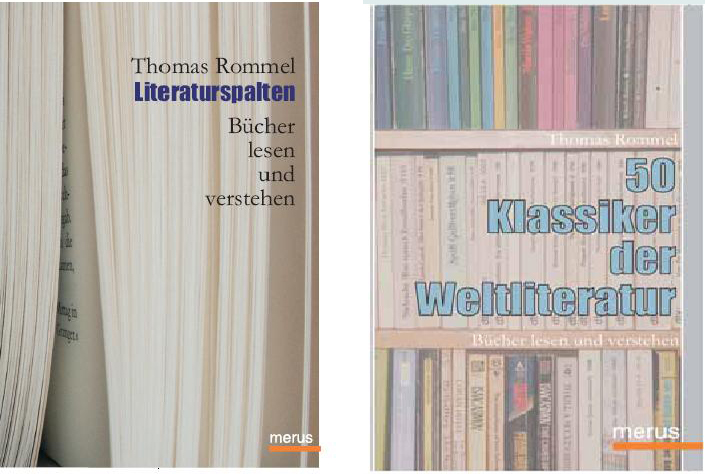
\includegraphics[width=0.8\textwidth]{./ArtLit/Rommel.jpg}
%   \mycaption{ xxx )}\label{fig:profxxx}
   \end{center}
\end{figure}






\vspace{0.6cm}
\textbf{Other Professional Activities}\\[-0.25cm]
\begin{enumerate}
\item[$\bullet$] Member of the Executive Committee of ALLC (Association for Literary and Linguistic Computing)
\item[$\bullet$] Member of INPUTS, Institut f�r postkoloniale und transkulturelle Studien, Universit�t Bremen
\item[$\bullet$] Co-editor of \textit{Prolepsis, the Heidelberg Review of English Studies.} With Richard Utz (University of Northern Iowa), Peter Paul Schnierer (Universit\"{a}t Heidelberg)
\item[$\bullet$] Vertrauensdozent, Studienstiftung des Deutschen Volkes
\item[$\bullet$] Board Member of Bremen Brain; Bremen Brain provides Bremen's scientists with a forum for interdisciplinary discussions and lectures. The aim is to improve Bremen's image and to organize different conferences using the contacts of BB-Members
\end{enumerate}




\vspace{0.6cm}
\textbf{PhD-Students}\\[-0.25cm]

Cansu \"{O}zmen\newline
\textit{American Travel Narratives in the 19th Century}\\[-0.15cm]

Mark Schreiber\newline
\textit{The Celtic Tiger on Stage and Screen. An Analysis of Contemporary Irish Theatre}\\[-0.15cm]

Beril Saydun\newline
\textit{Constructing Turkish Nationalism and Autobiographic Selves in Halide Edib's Works "Memoirs of Halide Edib, The Turkish Ordeal and Inside India"}\\[-0.15cm]

Susanne Puissant\newline
\textit{Irony and Satire in the Poetry of the First World War}\\[-0.15cm]
